\section{Auswertung}
\label{sec:Auswertung}

% \begin{figure}
%   \centering
%   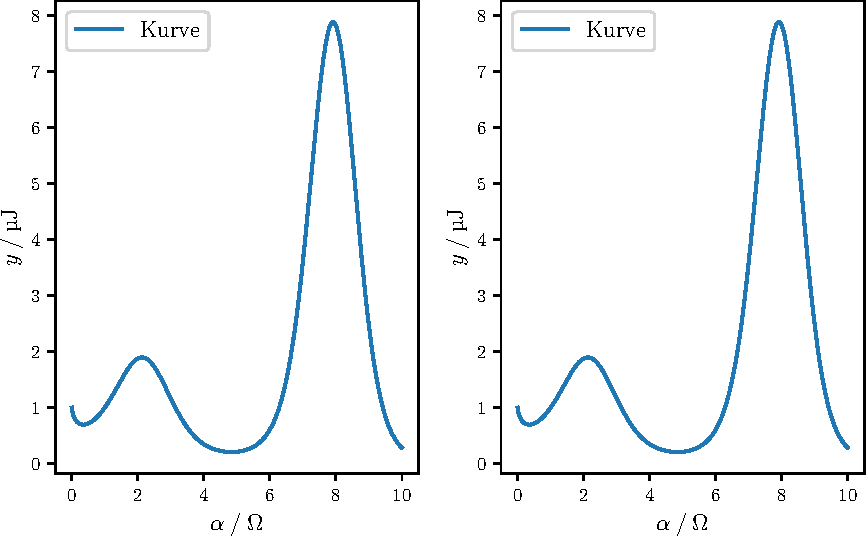
\includegraphics{plot.pdf}
%   \caption{Plot.}
%   \label{fig:plot}
% \end{figure}


\begin{table}[H]
  \centering
  \caption{Messwerte des zweiten Aufgabenteils bei 70 \% Leistung (6.000 rpm) des Gerätes.}
  \label{tab:Werte1}
  \begin{tabular}{c c c}
    \toprule
    Tiefe / $\si{\micro\second}$ & Signalstärke / $\SI{1000}{\square\volt\per\second}$ & Fließgeschwindigkeit / $\si{\centi\meter\per\second}$ \\
    \midrule
    12 & 5 & 181,5 \\
    12,5 & 6 & 124,2 \\
    13 & 7 & 39,8 \\
    13,5 & 8 & 44,6 \\
    14 & 13 & 50,9 \\
    14,5 & 16 & 54,1 \\
    15 & 20  & 60,5 \\
    15,5 & 10 & 73,2 \\
    16 & 7 & 66,9 \\
    16,5 & 10 & 66,9 \\
    17 & 11 & 57,3 \\
    17,5 & 6 & 57,3 \\
    18 & 9 & 44,6 \\
    18,5 & 7 & 50,9 \\
    19 & 7 & 54,1 \\
    19,5 & 7 & 54,1 \\
    20 & 6 & 60,5 \\
    \bottomrule
  \end{tabular}
\end{table}

\begin{table}[H]
  \centering
  \caption{Messwerte des zweiten Aufgabenteils bei 45 \% Leistung (3.870 rpm) des Gerätes.}
  \label{tab:Werte2}
  \begin{tabular}{c c c}
    \toprule
    Tiefe / $\si{\micro\second}$ & Signalstärke / $\SI{1000}{\square\volt\per\second}$ & Fließgeschwindigkeit / $\si{\centi\meter\per\second}$ \\
    \midrule
    12 & 4 & 342,2 \\
    12,5 & 5 & 79,6 \\
    13 & 6 & 38,2 \\
    13,5 & 7 & 28,7 \\
    14 & 8 & 28,7 \\
    14,5 & 9 & 28,7 \\
    15 & 14 & 30,2 \\
    15,5 & 17 & 30,2 \\
    16 & 16 & 31,8 \\
    16,5 & 12 & 28,7 \\
    17 & 16 & 27,1 \\
    17,5 & 11 & 25,5 \\
    18 & 8 & 25,5 \\
    18,5 & 7 & 28,7 \\
    19 & 8 & 28,7 \\
    19,5 & 8 & 31,8 \\
    20 & 6 & 36,6 \\
    \bottomrule
  \end{tabular}
\end{table}